\section{Dateisystem}\label{section:konzeption:dateisystem}

Nach \autoref{requirement:Integriertes Dateisystem} soll die IDE ein integriertes Dateisystem besitzen. Für dieses werden im Folgenden zunächst ein client-seitiger sowie ein server-seitiger Ansatz beschrieben.

Für den client-seitigen Lösungsansatz bietet sich eine Speicherung der Dateien des Nutzers innerhalb des Browsers an. Hierbei kann für die persistente Speicherung von Daten die Indexed Database API \cite{noauthor_indexed-database-api_nodate} genutzt werden. Diese wird von allen modernen Browsern unterstützt und erlaubt die langfristige Speicherung von größeren Datenmengen. Der Vorteil des client-seitigen Ansatzes ist die Tatsache, dass kein weiterer Speicherplatz für die Nutzer bereitgestellt werden muss, da die Daten auf deren Geräten gespeichert werden. Allerdings sind die Daten sowohl an die Domain der IDE, das Gerät des Nutzers als auch an den spezifischen Browser gebunden und müssen ggf. durch entsprechendes Exportieren und Importieren übertragen werden.

Der server-seitige Lösungsansatz basiert darauf, jedem Nutzer einen entsprechenden Speicherbereich zuzuteilen, in welchem seine Dateien gespeichert werden. Dies kann entweder über das Dateisystem des Servers oder über eine Datenbank geschehen. Der Vorteil dieser Art der Datenspeicherung liegt darin, dass sie unabhängig vom verwendeten Gerät und Browser ist. Allerdings wird für die Speicherung der Nutzerdaten entsprechender Speicherplatz auf dem Server benötigt, wodurch höhere Kosten und ein höherer Verwaltungsaufwand entstehen können. Zudem muss sichergestellt werden, dass das System nicht ausgenutzt werden kann.

Nach \autoref{requirement:Weitere Dateisysteme} soll die IDE die Anbindung weiterer Dateisysteme unterstützen. Laut Unteranforderung (a) soll daher ein entsprechender CrossLab-Service für die Bereitstellung und Nutzung von Dateisystemen entwickelt werden. Dieser soll dann nach Unteranforderung (b) von der IDE für die Anbindung weiterer Dateisysteme verwendet werden. Dementsprechend wird im Folgenden der \textit{Filesystem Service} beschrieben. Dateisysteme sollen die Erstellung von Ordnern und Dateien, das Lesen, Verschieben und Löschen dieser sowie das Schreiben von Dateien unterstützen. Zusätzlich soll auch die Existenz von Dateien und Ordnern überprüft sowie deren Eigenschaften abgefragt werden können. Weiterhin soll die Registrierung sogenannter \textit{Watcher} ermöglicht werden. Diese können von einem Filesystem Service Consumer für bestimmte Pfade registriert werden, um über Änderungen innerhalb dieser informiert zu werden. Der Filesystem Service Consumer besitzt Funktionen, um die einzelnen Operationen auszuführen, während der Filesystem Service Producer die Möglichkeit bietet, auf eingehende Anfragen zu reagieren und entsprechende Antworten an den Filesystem Service Consumer zu senden.

Nach \autoref{requirement:Teilen von Ordnern} soll das Dateisystem das Teilen von Ordnern mit anderen Nutzern innerhalb eines Experiments unterstützen. Dafür soll nach Unteranforderung (d) der bereits vorhandene Collaboration Service der IDE verwendet werden. Beim Erstellen eines Experiments öffnen Nutzer einen Raum zum Teilen ihrer Ordner. Das geteilte Objekt hat dabei die Kennzeichner der verschiedenen Teilnehmer als Schlüssel mit den geteilten Ordnern des jeweiligen Teilnehmers als den dazugehörigen Wert. Wenn ein Nutzer einen Ordner teilt, soll dieser anderen Nutzern angezeigt werden. Diese können dann den Inhalt einsehen und bearbeiten. Die Implementierung der Synchronisation ist hierbei abhängig von dem verwendeten Code Editor. Weiterhin kann über die Zustandsinformationen von Nutzern auch deren aktuelle Position mit den anderen Nutzern geteilt werden und diesen innerhalb der entsprechenden Datei angezeigt werden.

Für die Einbindung des Filesystem Service in die betrachtete Experimentkonfiguration kann ein Filesystem Service Consumer zur IDE hinzugefügt werden. Für die Bereitstellung von Dateisystemen können Laborgeräte einen entsprechenden Filesystem Service Producer anbieten. Ein Beispiel für ein derartiges Laborgerät ist ein Storage-Server, der es Nutzern ermöglichen könnte, ihre Dateien unabhängig von ihrem verwendeten Browser und Gerät speichern und abrufen zu können. Weiterhin kann die IDE auch einen Filesystem Service Producer zur Bereitstellung ihres integrierten Dateisystems anbieten. In \autoref{figure:experimentkonfiguration:dateisystem} ist die Erweiterung der betrachteten Experimentkonfiguration dargestellt. Dabei wurden sowohl ein Filesystem Service Consumer als auch ein Filesystem Service Producer bei den IDEs hinzugefügt.

\begin{figure}[tbp]
    \centering
    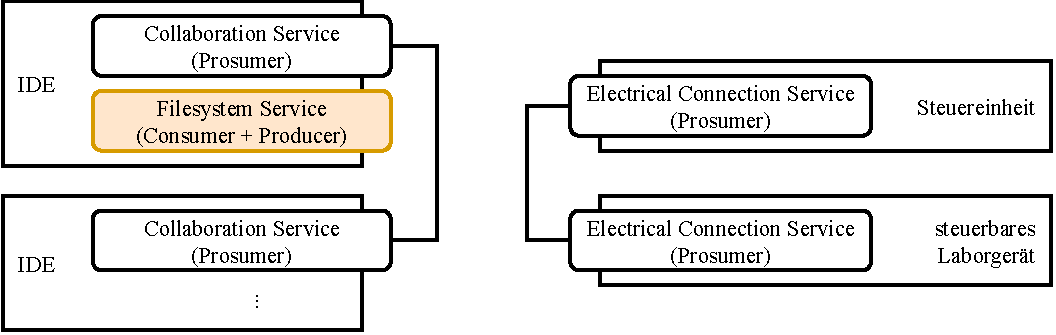
\includegraphics[width=\textwidth]{diagrams/experimentkonfigurationen/Experimentkonfiguration-02.drawio.pdf}
    \caption{Experimentkonfiguration (+ Dateisystem)}
    \label{figure:experimentkonfiguration:dateisystem}
\end{figure}